
\begin{tikzpicture}[x=0.75pt,y=0.75pt,yscale=-1,xscale=1]
	%Straight Lines [id:da0832972187828418] 
	\draw    (80,35) -- (185,35) ;
	\draw [shift={(188,35)}, rotate = 540] [fill={rgb, 255:red, 0; green, 0; blue, 0 }  ][line width=0.08]  [draw opacity=0] (5.36,-2.57) -- (0,0) -- (5.36,2.57) -- cycle    ;
	\draw [shift={(77,35)}, rotate = 360] [fill={rgb, 255:red, 0; green, 0; blue, 0 }  ][line width=0.08]  [draw opacity=0] (5.36,-2.57) -- (0,0) -- (5.36,2.57) -- cycle    ;
	%Straight Lines [id:da17602726868869878] 
	\draw    (80,70) -- (185,70) ;
	\draw [shift={(188,70)}, rotate = 540] [fill={rgb, 255:red, 0; green, 0; blue, 0 }  ][line width=0.08]  [draw opacity=0] (5.36,-2.57) -- (0,0) -- (5.36,2.57) -- cycle    ;
	%Straight Lines [id:da5151276494097119] 
	\draw    (80,105) -- (185,105) ;
	\draw [shift={(79,105)}, rotate = 360] [fill={rgb, 255:red, 0; green, 0; blue, 0 }  ][line width=0.08]  [draw opacity=0] (5.36,-2.57) -- (0,0) -- (5.36,2.57) -- cycle    ;
	
	% Text Node
	\draw (50,24) node [anchor=north west][inner sep=0.75pt]   [align=left] { \structure{{\Large\faUserSecret}} };
	\draw (200,24) node [anchor=north west][inner sep=0.75pt]   [align=right] {\structure{{\Large\faCat}}};
	\draw (102,15) node [anchor=north west][inner sep=0.75pt]   [align=center] {$P \in E(\mathbb{F}_q)$};
	% Text Node
	\draw (35,62) node [anchor=north west][inner sep=0.75pt]   [align=left] { \structure{$a \in \mathbb{N}$} };
	\draw (120,50) node [anchor=north west][inner sep=0.75pt]   [align=left] {$[a] P$};
	% Text Node
	\draw (120,86) node [anchor=north west][inner sep=0.75pt]   [align=left] {$[b]P$};
	\draw (190,98) node [anchor=north west][inner sep=0.75pt]   [align=right] { \structure{$b \in \mathbb{N}$} };
	% Text Node
	\draw (-40,130) node [anchor=north west][inner sep=0.75pt]   [align=left] {\structure{\boxed{[ab]P = [a]([b]P)}}};
	\draw (190,130) node [anchor=north west][inner sep=0.75pt]   [align=left] {\structure{\boxed{[ab]P = [b]([a]P)}}};
\end{tikzpicture}